\documentclass[apjl,twocolumn]{emulateapj}
\usepackage{graphicx}
\usepackage[varg]{txfonts}
\usepackage[pagebackref,breaklinks,colorlinks,citecolor=blue]{hyperref}        
\renewcommand*{\backref}[1]{[#1]}  % gives neat back references in the pdf
%\usepackage[%draft, 
%colorlinks,citecolor=blue,linkcolor=blue,urlcolor=blue]{hyperref}
\usepackage{aas_macros}
%\usepackage{amsmath} % clashes with emulateapjj for some reaons
\usepackage[usenames,dvipsnames]{xcolor}
\usepackage{comment}
\usepackage{multirow}
%\usepackage{chngpage}
%\usepackage{lscape}
\usepackage{url}
\newcommand{\todo}[1]{{\large $\blacksquare$~\textbf{\color{red}[#1]}}~$\blacksquare$}
\newcommand{\udef}{\stackrel{\mathrm{def}}{=}}
% for tree diagram
%\usepackage{forest}
%\usepackage{tikz-qtree}
%\usetikzlibrary{shadows,trees}

%Selma's comments
\definecolor{Wildstrawberry}{rgb}{1.0, 0.26, 0.64}
\newcommand{\SdM}[1]{{{\color{Sepia}{#1}}}}
\renewcommand{\SdM}[1]{{{{#1}}}}

\newcommand{\newtext}[1]{{\color{ForestGreen}\bf{#1}}}

\renewcommand{\labelitemii}{$\bullet$}
\newcommand{\kms}{{\,\mathrm{km\ s^{-1}}}}
\newcommand{\Msun}{{\,\mathrm{M}_\odot}}
\newcommand{\Lsun}{{\,\mathrm{L}_\odot}}
\newcommand{\masyr}{{\,\mathrm{mas}\,\mathrm{yr}^{-1}}}


\DeclareRobustCommand{\Eqref}[1]{Eq.~\ref{#1}}
\DeclareRobustCommand{\Figref}[1]{Fig.~\ref{#1}}
\DeclareRobustCommand{\Tabref}[1]{Table~\ref{#1}}
\DeclareRobustCommand{\Secref}[1]{Sec.~\ref{#1}}

\interfootnotelinepenalty=10000    % brute-forces the footnote not to break over two pages

  
\begin{document}

\title{Gaia identifies VFTS682 as the most massive % , dynamically
                                % ejected %% to fit in one line
  runaway star known to date}

\author{M.~Renzo$^{1}$, S.~E.~de~Mink$^{1}$, D.~J.~Lennon$^{2}$,
  S.~Justham$^{3,4}$, J.~Vink$^{5}$, F.~R.~Schneider$^6$,
  J.~Bestenlehner, A.~de~Koter$^{1}$ \todo{... add coauthors...} }

\affil{$^{1}$Astronomical Institute Anton Pannekoek, University of
    Amsterdam, 1098 XH Amsterdam, The Netherlands \\
    $^{2}$ ESA, European Space Astronomy Centre, Apdo. de Correos 78, E-28691 Villanueva de la Ca\~nada, Madrid, Spain \\
    $^{3}$ {School of Astronomy \& Space Science, University of the Chinese
    Academy of Sciences, Beijing 100012, China}\\
     $^4$ {National Astronomical Observatories, Chinese Academy of
       Sciences, Beijing 100012, China}\\
     $^5$ {Armagh Observatory, College Hill, Armagh BT61 9DG, UK}\\
     $^6$ {Department of Physics, University of Oxford, Keble Road, Oxford OX1 3RH, UK}  
}
  
\thanks{M.~Renzo, \href{mailto:m.renzo@uva.nl}{m.renzo@uva.nl}}
\date{}
\begin{abstract}
The formation and fates of the most massive stars remains one of the most elusive questions in stellar astrophysics. 
%
Previous spectroscopic studies identified VFTS682 as one of the most massive stars known. It resides in the field of the 30 Dor region in the Large Magellanic Cloud at a projected distance of 29\,pc of the star cluster R136. The lack of a detected offset in radial velocity derived from the spectra, lead to speculations whether such extreme stars can form in relative isolation. 
%
We use the unprecedented proper motions from the second Gaia data
release (DR2) to investigate the kinematics of this object. We show
that VFTS 682 is a bonafide runaway star moving with a relative
velocity of about $64\pm21\kms$ away from the star cluster R136.  The
inferred age, distance, and the magnitude and direction of the
velocity are consistent with a dynamical ejection scenario from the cluster. 
%
This would make VFTS 682 the most massive runaway star known to date.  It proves that star clusters are capable of ejecting their most massive members. We discuss the implications for the existence of stars with masses well above $100\Msun$ inside the cluster, the internal dynamics in dense star clusters and the final fate of this object. 

\end{abstract}

\keywords{stars: kinematics, stars: runaways, stars: individual: VFTS682}
\maketitle{}

\section{Introduction}
\label{sec:intro}

How do massive stars form is one of the major longstanding questions in astrophysics
\citep[e.g.,][]{zinnecker:07}. Obtaining clues from observations has been challenging, because massive stars are intrinsically rare, 
%\citep[e.g.,][]{salpeter:55,kroupa:01, schneider:18}, 
evolve fast, typically reside in dense groups and they remain enshrouded in their parent cloud during the formation
process.  Major progress has been made on the theoretical side,
\citep[e.g.][]{kuiper:15,rosen:16}, but simulations cannot yet resolve
the smallest length scales that are of interest to understand the 
high level of multiplicity among massive stars  \citep[e.g.,][]{bate:09, sana:17}.  Understanding massive star formation, and its
possible dependence on environment and metallicity, is crucial for
understanding the role massive stars play within their host galaxies
as sources of feedback, but also for understanding the transients that
mark their death and the compact remnants they leave behind.  This is
therefore a key question for the present and upcoming transient
surveys e.g., Large Synoptic Spectroscopic Survey and LIGO/Virgo,
%\citep[][]{}\todo{ref} . Blackgem is still hypothetical and a very tiny project compared to the others.  
which  will reveal transients associated to massive stars
evolution and death.

In has been proposed that most, if not all, stars form in clusters \citep{lada:03}, where massive stars are thought to  form preferentially in the dense cores of clusters. In this picture, field stars are primarily the result of the dissolution of dense groups. 
However, a significant population of massive stars exists in relative
isolation,  far from dense clusters or OB associations. The origin of
this population still remains debated \citep{lamb:16,ward:18}.   One
hypothesis is that they  formed in the field, but this poses a
challenge for the theories of star formation. The alternative
hypothesis is that these massive stars formed in clusters, and then
been ejected from their birth locations. Such ejections may result
from dynamical interactions \citep[e.g.,][]{poveda:67} or from the disruption of binary systems by the core-collapse of the companion star \citep[e.g.,][]{zwicky:57, blaauw:61}. 
 
An interesting contribution to the debate on whether or not massive
stars an form in relative isolation was presented by
\cite{bestenlehner:11, bressert:12}, who discuss the case of the very massive star
VFTS682.   This star is located in the field of the 30 Doradus region
in the Large Magellanic Cloud (LMC) and was studied as part of the
multi-epoch spectroscopic VLT-FLAMES Tarantula Survey (VFTS) of
massive stars \citep{evans:11}.  Its spectral type is WNh5 and its 
present-day mass is $137.8^{+27.5}_{-15.9}\,M_\odot$,
\citep{schneider:18}. These correspond to an inferred initial mass of
$150.0^{+28.7}_{-17.4}\,M_\odot$ and a wind mass loss rate of
$\sim10^{-4.1\pm0.2}\,M_\odot \ \mathrm{yr}^{-1}$ inferred from the
spectral analysis not accounting for clumping
\citep[][]{bestenlehner:11}, which make it one of the
most extreme objects in the region.  It is reminiscent of the very
massive stars % , a.k.a. ``monster stars'',
identified by
\citet{crowther:10, crowther:16} in the core of the
R136 cluster. 
 
Most remarkable is the location of VFTS682, at a projected distance of
$\sim$$29$\,pc from the core of the star cluster
R136. \citet{bestenlehner:11} discuss two possibilities for the
origin of VFTS 682. Quoting directly from their abstract: "either (i) the star either formed in situ, which would have profound implications for the formation mechanism of massive stars, or (ii) VFTS 682 is a slow runaway star that originated from the dense cluster R136, which would make it the most massive runaway known to date."

In this study we report on our analysis the data from the second Gaia data release (DR2) \cite[][]{gaia:16,brown:18}.  We combine the radial velocity measurements from the VFTS survey \citep[][]{evans:11} with the proper motion from Gaia DR2 to reconstruct the three-dimensional velocity of VFTS682, and test the hypothesis that this star was ejected from R136. 

Our results indicate that VFTS 682 is a bona fide runaway star.  The direction and magnitude of the velocity vector is fully consistent with dynamical ejection from R136.  Its inferred age is consistent with the inferred travel time. This means that the hypothesis that VFTS 682 is formed in relative isolation is rejected.  This makes VFTS 682, with an inferred present day mass well above a hundred solar masses, the most massive runaway star known to date. 


\section{Observations}
\label{sec:sample}

% feels like unnecessary here...
% In this section we summarize the remarkable properties derived for VFTS682 \todo{?}\Secref{data:vfts683}
% in earlier studies and we discuss we Gaia data in \Secref{data:gaia}.

\subsection{ Overview of VFTS682 from previous studies \label{data:vfts683}}

The star VFTS682  \citep{evans:11}, located at right ascension (RA)
05$^\mathrm{h}$38$^\mathrm{m}$55.510$^\mathrm{s}$  and declination
(DEC) -69:04:26.72 in the ICGS frame \citep[][]{brown:18}
was originally classified as a young stellar object \citep{gruendl:09}
based on its mid-infrared excess.  \citet{evans:11} classified the
object as Wolf-Rayet star of spectral type WNh5 using spectra from the
VFTS survey.  The spectra available covered $\lambda$4000--7000 and
were taken at multiple epochs. Using the same dataset,
\citet{bestenlehner:11} excluded the presence of a close companion
with high confidence from the absence of radial velocity variations.

\citet{bestenlehner:11} further analyzed the spectra using the non-LTE
model atmosphere code CMFGEN \citep{hillier:98} to derive the stellar
parameters and surface abundances. They inferred a peculiar extinction
($R_V\simeq4.7$), leading to a surprisingly high luminosity
$\log_{10}(L/L_\odot) =  6.5\pm0.2$. \citep{schneider:18} estimated
the present-day mass of VFTS682 at  $137.8^{+27.5}_ {-15.9}\Msun$, an
apparent age of $1.0^{+0.2}_{-0.2}$\,Myr and an inferred initial mass
of $150.0^{+28.7}_{-17.4}\Msun$, using the Bayesian analysis tool Bonnsai
\citep{schneider:17}, based on the evolutionary models from
\citet{brott:11, kohler:15}. These values place VFTS682 around the
``canonical upper limit'' of $\sim$$150\Msun$ by \citet{figer:05}.

The star is very similar from the spectral point of view to R136a3, located inside the star cluster
R136, \citep{crowther:10}  for which \citet{crowther:16} report a
current mass estimate of $180^{+30}_{-30}\Msun$. The R136 cluster hosts
at least two more very massive WN5h stars R136a1, R136a2 whose
estimated current masses are even higher. However, VFTS682 stands
out by its isolation at a projected offset of 29\,pc from the center
of the cluster \citep{bestenlehner:11}.  

Further worth noticing is the variability of the star.
\citep{bestenlehner:11} discuss the Optical Gravitational Lensing
Experiment (OGLE-III) light curves \citep{udalski:08} and show a
variability in the V-band of the $\sim$10\% level on a timescale of years.
The comment that this is unusual for Wolf-Rayet and more reminiscent
of Luminous Blue Variable (LBV) stars. 

\todo{Report mass loss rate.  Report LOS velocity.}
\citep{parker:93}

\subsection{New data from Gaia DR2  \label{data:gaia}}

\begin{table}[t]
\begin{center}
    \caption{Astrometric parameters for VFTS682. }
%
  \begin{tabular}{l|c|c}
  \tableline
\tableline
    Parameter & Value & Source\\ 
    \tableline
    RA \hfill[degree] &  \phantom{-}84.73 $\pm$  0.03 & \multirow{4}{*}{Gaia DR2}\\
    DEC \hfill [degree] & -69.07 $\pm$  0.05  & \\
    $\mu_\mathrm{RA}$  \hfill[$\mathrm{mas\ yr^{-1}}$] & \phantom{-0}1.84 $\pm$ 0.07 & \\
    $\mu_\mathrm{DEC}$  \hfill[$\mathrm{mas\ yr^{-1}}$] & \phantom{-0}0.78 $\pm$ 0.08& \\
    $\delta v_\mathrm{rad}$  \hfill[$\kms$] & \phantom{0}-45 $\pm$ 25 & \cite{bestenlehner:11}\\
\tableline
  \end{tabular}
  \tablecomments{The peculiar radial
    velocity $\delta v_\mathrm{rad}$ is obtained as the difference
    between the average radial velocity of the 30 Doradus region
    ($270\pm10\kms$) minus the radial velocity measured from the HeII $\lambda4686$
    line for VFTS682 ($315\pm15\kms$).}
    \end{center}
  \label{tab:vfts682}
\end{table}

% %% Any table notes must follow the \end{tabular} command.

% %%% change \tablenotetext{a} - \tablenotetext{1} etc. to omit LaTeX errors
% %%% Karol Kozio? for ShareLaTeX


The Gaia Data Release 2, which became available on 25 April 2018,
provides the five-parameter astrometric solution (positions,
parallaxes, and proper motion components) for more than a billion
sources \citep{brown:18}.%  \todo{why do we care about the
%   median? I'm
%   selecting data with errors smaller than this, and I'm not using
%   fainter stars!I think this is not useful here} The median uncertainty in the proper motion
% components the corresponding uncertainties are $0.05\,\masyr$ for
% bright sources  ($G<14$ mag) and $0.2\masyr$ at $G=17\,\mathrm{mag}$
% \citep{lindegren:18}.  The uncertainties quoted above correspond to $xx\kms$ and $yy\kms$ respectively.  This unprecedented accuracy allows the identification of bright runaway stars at the distance to the LMC, 50\,kpc. 

VFTS682 is identified with the id 4657685637907503744 in the Gaia DR2
catalog\footnote{\url{https://vizier.u-strasbg.fr/viz-bin/VizieR-3?-source=I/345/gaia2}}. Gaia
reports a G-band magnitude of 15.65. The star has a
\texttt{visibility\_period} = 17, which counts how many observations have
been used to reconstruct its astrometric solution
\citep[][]{lindengren:18}, and the reported
\texttt{astrometric\_excess\_noise} = 0. These values suggest that the Gaia
data for VFTS682 are reliable. However, the effective temperature
reported in Gaia DR2 is one order of magnitude lower than what found by
\cite{bestenlehner:11}, and the best fit parallax of this star is
negative. We do not use the effective temperature of the star anywhere
in this study, and we attribute the unphysical value of the parallax
to the large distance to the LMC. Our main findings do not rely on the
parallax nor the effective temperature values reported in the Gaia DR2
catalog.

We retrieve for VFTS682 the position in RA and DEC
in the IGCS frame \cite[][]{brown:18}, its
proper motion components ($\mu_\mathrm{RA}$, and $\mu_\mathrm{DEC}$,
respectively). For the radial velocity of VFTS682 and of the 30 Doradus
region as a whole, we instead use the VFTS data
as quoted in \cite{bestenlehner:11}. \Tabref{tab:vfts682} lists the values adopted throughout
this work for each of these quantities.


We define a local standard frame of reference to derive the peculiar velocity
of VFTS682 by selecting from the Gaia DR2 catalog a sample of nearby
stars, following closely the approach of \cite{lennon:18}.
We select all the stars in a target of 0.2 degrees around R136
(NGC2070) fulfilling the following criteria. First, we require G-band
magnitude brighter than 17, correspondingly roughly to the
completeness level of the VFTS survey \citep[here we implicitly assume
G$\sim$V,][]{evans:11}. Then we require \texttt{visibility\_period} $\geq$ 5,
\texttt{astrometric\_excess\_noise} $< 1$, the errors on the proper
motion components to be smaller than 0.1\,$\mathrm{mas\ yr^{-1}}$,
and the proper motion components themselves to be smaller than
2\,$\mathrm{mas\ yr^{-1}}$ in absolute value. At the distance to the
LMC, $1\mathrm{mas\ yr^{-1}}\simeq250\,\kms$ \citep[e.g.,][]{lennon:18}, so the cut on the values
of the proper motions removes stars that would have projected
tangential velocities in excess of $\sim$500\,$\kms$, which are most
likely to be foreground stars. We checked that the additional
requirement of having parallaxes smaller than $2\,\mathrm{mas}$ does
not reduces further our sample. 

We calculate the averaged proper motion components for the whole
region using 
\begin{equation}
  \label{eq:mean}
  \langle \mu_i\rangle = \frac{\sum_\mathrm{stars}\frac{1}{\Delta
      \mu_i}\mu_i}{\sum_\mathrm{stars} \frac{1}{\Delta \mu_i}} \ \ , \
  \ \Delta \langle \mu_i\rangle = \frac{\sqrt{N}}{\sum_\mathrm{stars}
    \frac{1}{\Delta \mu_i}} \ \ ,
\end{equation}
where $i = \mathrm{RA}, \mathrm{DEC}$, and $\Delta \mu_i$ is the error
on the proper motion component reported by Gaia. The sums run over
all the $N=651$ stars in our selected sample. We evaluate each proper motion
component separately. For simplicity, throughout this study, we assume the same
distance of $50$\,kpc to the star \citep[][]{pietrzynski:13}, and to
the 30 Doradus region as a whole. We do not consider the error bars on
the distance determination when converting proper motions into
physical velocities. The data retrieved, and the ipython notebook used for the analysis
presented here will be made available at \todo{probably git repo on bitbucket?}. 

\section{The kinematics of VFTS682}
\label{sec:results}

\subsection{Is it a runaway star?}
\label{sec:runaway}
We first address the question of whether VFTS682 is a typical star
from the kinematic point of view, or whether it is a runaway star with
a significantly large peculiar velocity compared to its surrounding population. The former is what should
be expected if it formed where we observe it today, in relative
isolation from other massive stars.

Using the 651 stars selected as described in \Secref{data:gaia} (a
subset is shown in blue in \Figref{fig:main}), we find averaged proper motion components of
$\langle\mu_\mathrm{RA}\rangle = 1.683\pm0.002\,\mathrm{mas\ yr^{-1}}$ and
$\langle\mu_\mathrm{DEC}\rangle =
0.672\pm0.003\,\mathrm{mas\ yr^{-1}}$. We note that these values are
in good agreement with what is found by \cite{lennon:18}. Subtracting these values from the
proper motions of VFTS682 (see \Tabref{tab:vfts682}), we obtain the
components of proper motion of the star relative to the surrounding region
$\mu_\mathrm{RA} = 0.16\pm 0.07\,\mathrm{mas\ yr^{-1}}$ and $\mu_\mathrm{DEC} =
0.11\pm 0.08\,\mathrm{mas\ yr^{-1}}$. We note that the error budget is
dominated by the errors on the proper motion components of VFTS682.

These can be converted in the
the components of the relative transverse velocity $\delta v_\mathrm{RA}=38\pm17\,\kms$,
$\delta v_\mathrm{DEC}=26\pm19\,\kms$, assuming a distance of
50\,kpc. % (we do not account for the uncertainty in the distance
% estimate when propagating errors).
The radial velocity from
\cite{bestenlehner:11} then gives the third component along
the line of sight, allowing us to calculate the three-dimensional
peculiar speed of the star:

\begin{equation}
  \label{eq:speed_around}
  v_\mathrm{pec} = \sqrt{\left(\delta v_\mathrm{RA}\right)^2
    +\left(\delta v_\mathrm{DEC}\right)^2+\left(\delta
      v_\mathrm{rad}\right)^2} = 64 \pm 21 
  \, \kms \ .
\end{equation}
This value for the three-dimensional speed of VFTS682 with respect the
surrounding stars make it the most massive ``bona fide'' runaway star
known to date.

\subsection{Does it come from the R136 cluster?}
\label{sec:r136_origin}

The red arrow in \Figref{fig:main} shows the proper motion of VFTS682
relative to the region, and the lighter red arrows show the possible
range of directions within the uncertainties in the measured proper
motion. It is clear that the most likely origin of the star is R136,
as suggested based on numerical N-body simulations by \cite{fujii:11, banerjee:12}.

%\subsection{Kinematic age}

We can therefore consider the kinematic age for this star assuming
that it originates from the cluster,

\begin{equation}
  \label{eq:kin_age}
  \tau_\mathrm{kin} = \frac{d_\parallel}{v_\parallel} \simeq
  \frac{29\,\mathrm{pc}}{46\,\kms} \simeq 0.6\pm\,0.2 \mathrm{Myr} \ \ ,
\end{equation}
where $d_\parallel =29$\,pc is the projected distance from VFTS682 to
the core of R136 \citep[][]{bestenlehner:11}, $v_\parallel \equiv \sqrt{\left(\delta v_\mathrm{RA}\right)^2
    +\left(\delta v_\mathrm{DEC}\right)^2} =46\pm
17\,\kms$ is the speed of the star relative to the cluster projected on the sky, obtained
using the relative proper motion components calculated in
\Secref{sec:runaway}, and we use the approximation $1 \kms \simeq 1
\mathrm{pc \ Myr^{-1}}$. As in the rest of this study, we neglect for
simplicity the error on the distance estimates.

The kinematic age $\tau_\mathrm{kin}$ is smaller than the apparent age
of the star age of $1.0\pm 0.2$\,Myr from \cite{schneider:18}, which
corroborates the idea that the star is the result of a dynamical
ejection. 

\begin{figure}[htbp]
  \centering
  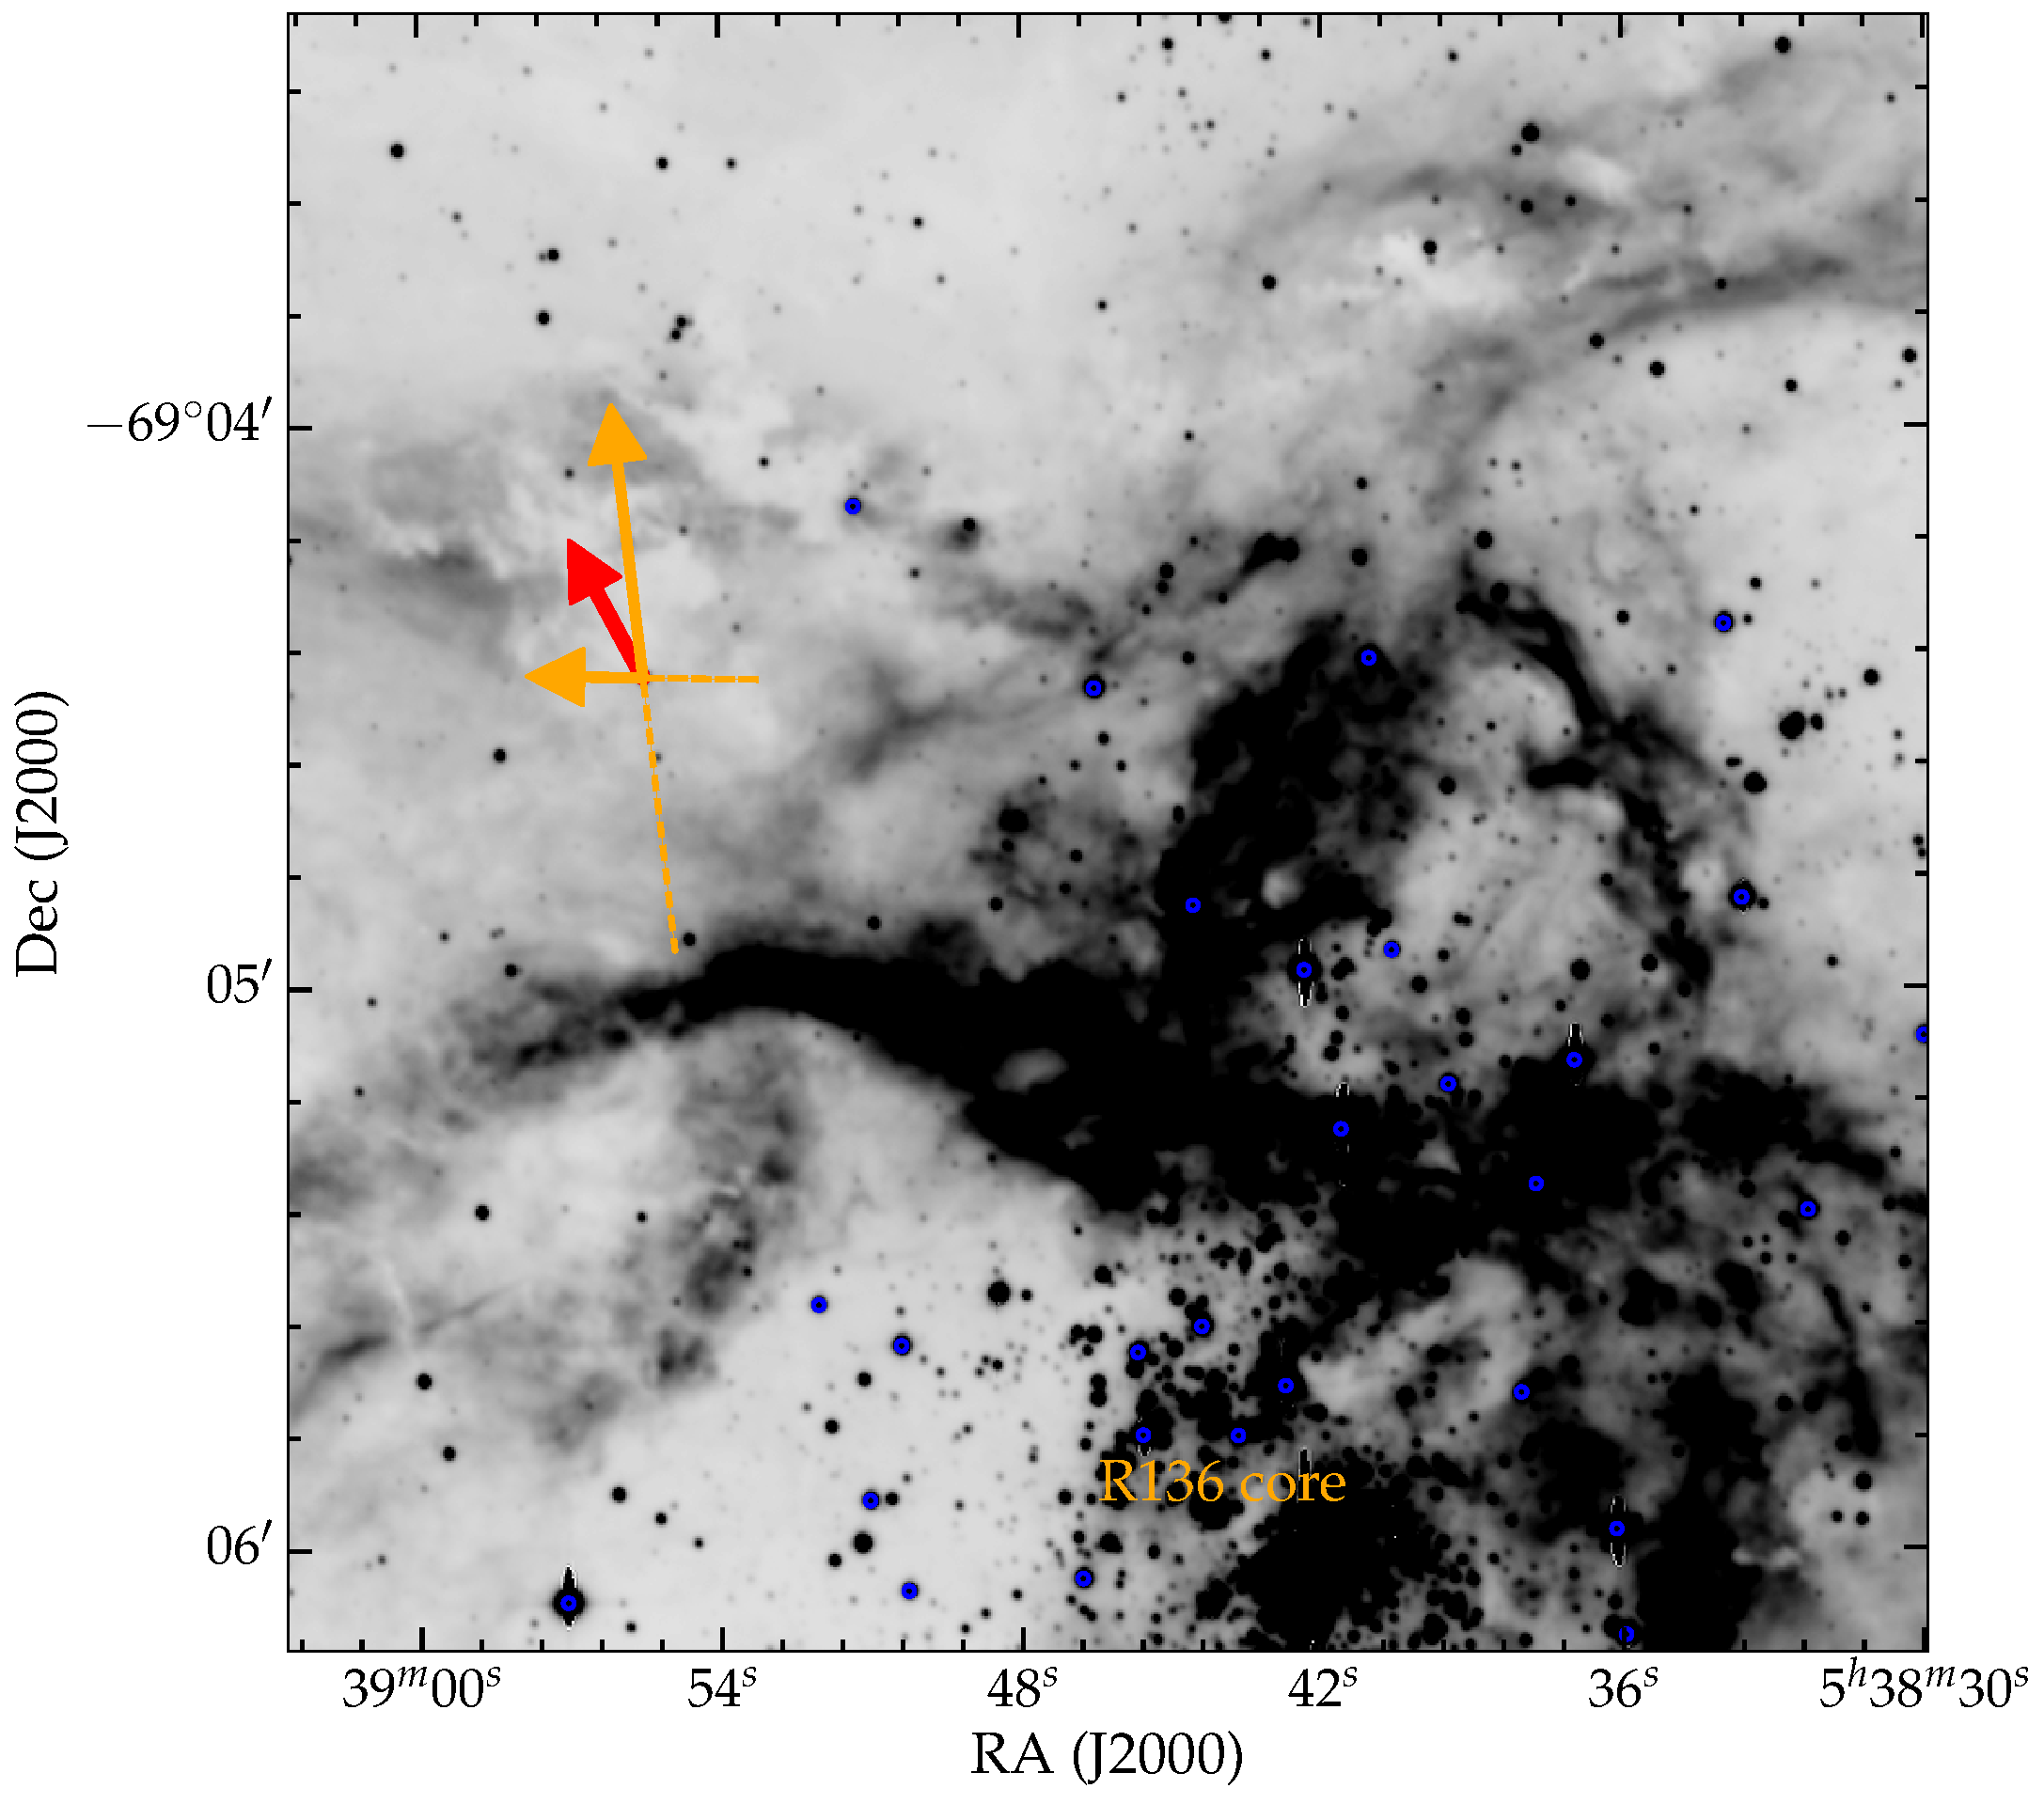
\includegraphics[width=0.5\textwidth]{./figures/main_plot_good}  
  \caption{The red solid arrow indicates the proper motion of VFTS682
    relative to the region, starting from the present day position of
    the star. The semi-transparent arrows indicate the possible
    directions of projected motion within the errors, and are extended
    backwards to illustrate the uncertainty on the origin of the
    star. The blue stars
    are a subset of those we use to define the local rest frame. \todo{load color picture on background}}
  \label{fig:main}
\end{figure}

\section{Discussion}
\label{sec:discussion}
\todo{Selma: Should add caveat that it may be a spurious detection.  That reconfirmation in following epochs is warranted. }

Based on our results, we can claim that VFTS682 is the most massive
runaway known to date, with a peculiar three-dimensional speed of $64\pm21\,\kms$. This means that isolated star formation is
\emph{not} required to explain this star. Its proper motion suggests that it was ejected from the cluster R136
$0.6\pm0.2$\,Myr ago. Because of the exceptionally large mass
of this star, this raises the question of which stars must populate
the core of the cluster.

Dynamical ejections due to N-body interactions typically (although, not necessarily) eject the least
massive star among those interacting \todo{ref}. This means that, just
based on the kinematic properties of VFTS682, we would expect several
stars with initial masses larger than $\sim$$150\,M_\odot$ in the
cluster R136.
This is consistent with the detection
of extremely massive stars by \cite{crowther:10} in the core of the
cluster. The projected rotational equatorial
velocity\footnote{However, the determination of the rotational
  velocity for stars showing lines in emission is complicated because
  of the optically thick wind screening the surface of the star, and should be
  considered with caution.} of VFTS682
reported by \cite{schneider:18} is $v\sin(i)<200\,\kms$, which is in
line with the average rotation rate of massive stars in the region
\citep[][]{ramirez-agudelo:15}. This suggests that VFTS682 (i) has not
experienced rotationally induced chemically homogeneous evolution
\citep[][]{maeder:00,demink:09,marchant:16}, and (ii) it has not
accreted mass from a binary companion, nor it will, since the multi-epoch
data of the VFTS survey rule out the presence of a companion at
present day. Moreover, the spectral type of VFTS682
\citep[WNh5,][]{bestenlehner:11} is the same as R136a1-a3, i.e.~the
three most massive stars detected in the core of the cluster by
\cite{crowther:10}, with an astonishing similarity in particular with
the spectrum of R136a3. Therefore,
VFTS682 might be an ideal target to constrain the stellar physics of
stars with masses well above $\sim$$100\,M_\odot$: its isolation makes
it an easier target for observations compared to the similar stars
present in the crowded core of R136.

The similarities between VFTS682 and the WNh5 stars in the core of
R136 are also in agreement with the ``bully binary'' model of
\cite{fujii:11}. Based on their numerical results, they suggested that
early in the evolution of a cluster, dynamical interactions form an extremely
massive binary, which then tightens its orbit by ejecting other stars passing
by. Interpreting our results for VFTS682 through the lens of their simulations
suggests the presence of a binary with total mass
$M_1+M_2\gtrsim 300\,M_\odot$ in the core of the cluster. Such bully
binary could be R145 according to \cite{fujii:11}.

The kinematic age of VFTS682 puts an
upperlimit to the timescale to form such ``bully binary'' in
R136. The cluster must have been at the very beginning of its
evolution, given the age estimate of $\lesssim 2$\,Myr
\cite{crowther:10,sabbi:12} and the kinematic age of VFTS16. If the
cluster is indeed younger than the shortest stellar lifetime
\citep[$\sim$3\,Myr, e.g.,][]{zapartas:17}, ejection from a binary
system of VFTS682 is excluded since the region is to young for stars
to have experience core-collapse already.

\todo{check \cite{banerjee} and rewrite next paragraph, they
  have stuff} Unfortunately, their simulations did not include stars more
massive than $100\,M_\odot$, so it is difficult to predict, based on
the existence of VFTS682, how many other stars should have been
ejected from the cluster already and what is their mass
distribution. A comprehensive study of the kinematic properties of the
large sample of stars with extremely large inferred masses visible
around R136 is encouraged.  

\cite{lennon:18} have carried out a similar study on VFTS16, another
massive star ($\sim90\,M_\odot$) in the 30 Doradus region, previously
known to be a runaway from the value of
its radial velocity. They also concluded that VFTS16 is 
the result of a dynamical ejection from the R136 cluster. 
The value of $\tau_\mathrm{kin}\simeq0.63$\,Myr we find for VFTS682 (see \Secref{sec:r136_origin}) is smaller
than the corresponding value for VFTS16: \cite{lennon:18} inferred a kinematic age of
$\sim$1.5\,Myr, possibly in tension with the apparent age of that star. This means that the more
massive VFTS682 was ejected later than VFTS16 from the same cluster.



\begin{itemize}
\item is R136 a single young cluster or a merger
\item estimate the influence of the gravitational potential of R136,
  what is its total mass and relaxation time?
\item Make link to dynamical interaction proposed to form BHBH
  systems.
  \item from Fabian's email (see comment in tex):% One last aspect: I am always wondering what happens to the star/binary that ejected 682. There is a huge linear momentum in this star of ~150 Msun * 60 km/s. Even if the bully was a 300 Msun total object, it would obtain a kick of 30 km/s. Is this enough to eject the bully star? This velocity would already be 100 km/s for a 90 Msun bully (I was thinking of 016 here... 'Cause I do not know what ejected this object either). Of course, if there is a third body, these velocities are no longer correct. The escape velocity from R136 at 0.5pc for a total mass of 10^5 Msun would only be of order 20 km/s... So a 300 Msun bully is at the edge of what is possible and one might need something even more massive or another very massive object will also be ejected. Or am I wrong here? Do the Banerjee and Co simulations say something about this?
\end{itemize}



% \todo{Merge Selma's my\_bib bibtex file with Mathieu's and prevent
% double refs. } %% copied everything in one file

\bibliographystyle{aa}
\bibliography{bibliography/vfts682}

\begin{acknowledgements}
  \small
  We are grateful to S.~Torres for 
  very useful discussions on the
  Gaia DR2 dataset, and to M.~C.~Ramirez-Tannus for invaluable help.
  SdM has received funding under the European Unions Horizon 2020 research and innovation programme from the European Research
  Council (ERC) (Grant agreement No. 715063).
  This work has made use of data from the ESA space mission Gaia (\url{http://www.cosmos.esa.int/gaia}), processed by the Gaia Data Processing and Analysis Consortium (DPAC, \url{http://www.cosmos.esa.int/web/gaia/dpac/consortium}). Funding for the DPAC has been provided by national institutions, in particular the institutions participating in the Gaia Multilateral Agreement. 
  The background image of \Figref{fig:main} is based on observations
  made with ESO Telescopes at the La Silla Observatory under programme
  ID 076.C-0888, processed and released by the ESO VOS/ADP group.
  This research made use of APLpy, an open-source plotting package for Python \citep[][]{robitaille:12}.
\end{acknowledgements}

\end{document}




%%% Local Variables:
%%% mode: latex
%%% TeX-master: t
%%% End:
